

\chapter{Social connectedness index II from Facebook}

\resp{Miguel Avilés Moreno}



\section{Introduction}

This project focuses on the analysis of the Facebook Social Connectedness Index (SCI) of October 2021 to study the global structure of social ties. The dataset provides a scaled measure of social connections between pairs of geographic areas, including NUTS3 regions in Europe and GADM regions elsewhere. Our objective is to build a network of the top 100 countries (excluding the USA) where nodes represent GADM NUTS3 areas and edges encode friendship intensity between regions. The project involves generating two output files: one containing node information and another containing the edge list. Finally, we will perform a simplified network analysis to compare structural properties across countries.

The Social Connectedness Index (SCI) is a measure derived from anonymized Facebook data that quantifies the intensity of social ties between pairs of geographic areas. 

\section{Data Description}

For this analysis was used the dataset from~\cite{facebook2025sci}, which provides the SCI as of October 2021. The main file, \texttt{gadm1\_nuts3\_counties-gadm1\_nuts3\_counties - FB Social Connectedness Index - October 2021.tsv}, contains pairwise connections between geographic regions, including each area's connections to itself. Each row records a pair of locations and the scaled SCI value. The second file provides the administrative level and type of each location code, facilitating interpretation of the regional identifiers, \texttt{gadm1\_nuts3\_counties\_levels.csv}.

\section{Nodes File}

To prepare the list of nodes, we excluded all connections involving the United States. From the rest of countries, we identified the top 100 with the highest number of unique regional nodes.

After selecting this subset, we retained only the locations appearing in pairs where both ends belonged to the same country, ensuring a consistent national context for the connections. 

To locate the node, we retrieved geographical coordinates (longitude and latitude) corresponding to each region. For European NUTS3 regions, we used centroid coordinates derived from the Eurostat shapefiles dataset~\cite{eurostat2025nuts}. For GADM regions, we relied on version 2.5 of GADM boundaries included in the original data repository~\cite{facebook2025sci}. Because GADM codes in Facebook’s dataset do not always match GADM’s standard notation, we obtained consistent centroids defining a conversion function and the assistance of Gemini~\cite{google2025gemini}. 

\section{Edges File}

The edges represent the social connections between pairs of regional nodes. To avoid trivial loops, we removed all self-links (where a region connects to itself) and ensured that each pair of nodes was counted only once, eliminating duplicate entries arising from undirected network records.

Since nearly all region pairs have some level of social connectedness (with a strictly positive SCI), including every link would result in a fully connected graph with very high density, offering limited interpretive value. Therefore, we applied a threshold: for each country, we computed the mean SCI across all its internal pairs and retained only edges whose SCI exceeded this mean, improving the relevance of subsequent analyses. The resulting edge list includes the identifiers of the source and target nodes, the country to which the link belongs, and the scaled SCI value quantifying the strength of the connection.


\section{Network Analysis of Top Countries}

In this section, the aim is to assess the structure and connectivity of the different regions within a country. The table below show a slice of the countries results for the metrics computed (Number of Nodes, Number of Edges, Network Density, Average Path Length, Clustering Coefficient and Number of Components).




We see that countries such as India and Canada have large networks with a high number of nodes and edges. Hong Kong exhibits a very dense and well-connected network with a high clustering coefficient, despite its relatively small number of nodes. Countries like Argentina show sparse networks, with low density and few edges.


As illustrated in Figure~\ref{fig:network-structure}, we observe a clear positive relationship between the number of nodes and the number of edges in national networks.

\section{Degree Distribution and Network Topology}

We performed an analysis of the degree distribution and network topology for two countries: Serbia (RS) and India (IND). The results show that India's network exhibits a higher average node degree, indicating dense interconnections across regions. In contrast, Serbia's network is relatively sparse, with fewer regional links and lower node connectivity overall. These structural differences are visually represented in Figure~\ref{fig:combined_network_analysis}.







\newpage
\section*{Supplementary Materials}

\begin{table}[H]
\centering
\footnotesize
\begin{tabular}{lrrrrrr}
\toprule
\textbf{Country} & \textbf{\#Nodes} & \textbf{\#Edges} & \textbf{Density} & \textbf{Avg. Path} & \textbf{Clustering} & \textbf{\#Components} \\
\midrule

ARG & 24 & 3 & 0.0109 & 1.00 & 0.000 & 5 \\
CAN & 293 & 2188 & 0.0511 & 4.24 & 0.185 & 1 \\
IND & 644 & 8717 & 0.0421 & 3.67 & 0.211 & 2 \\
HKG & 18 & 69 & 0.4510 & 1.57 & 0.579 & 1 \\
\bottomrule
\end{tabular}
\caption{Sample of network metrics for selected top countries.}
\label{tab:network_metrics}
\end{table}


\begin{figure}[htbp]
  \centering
  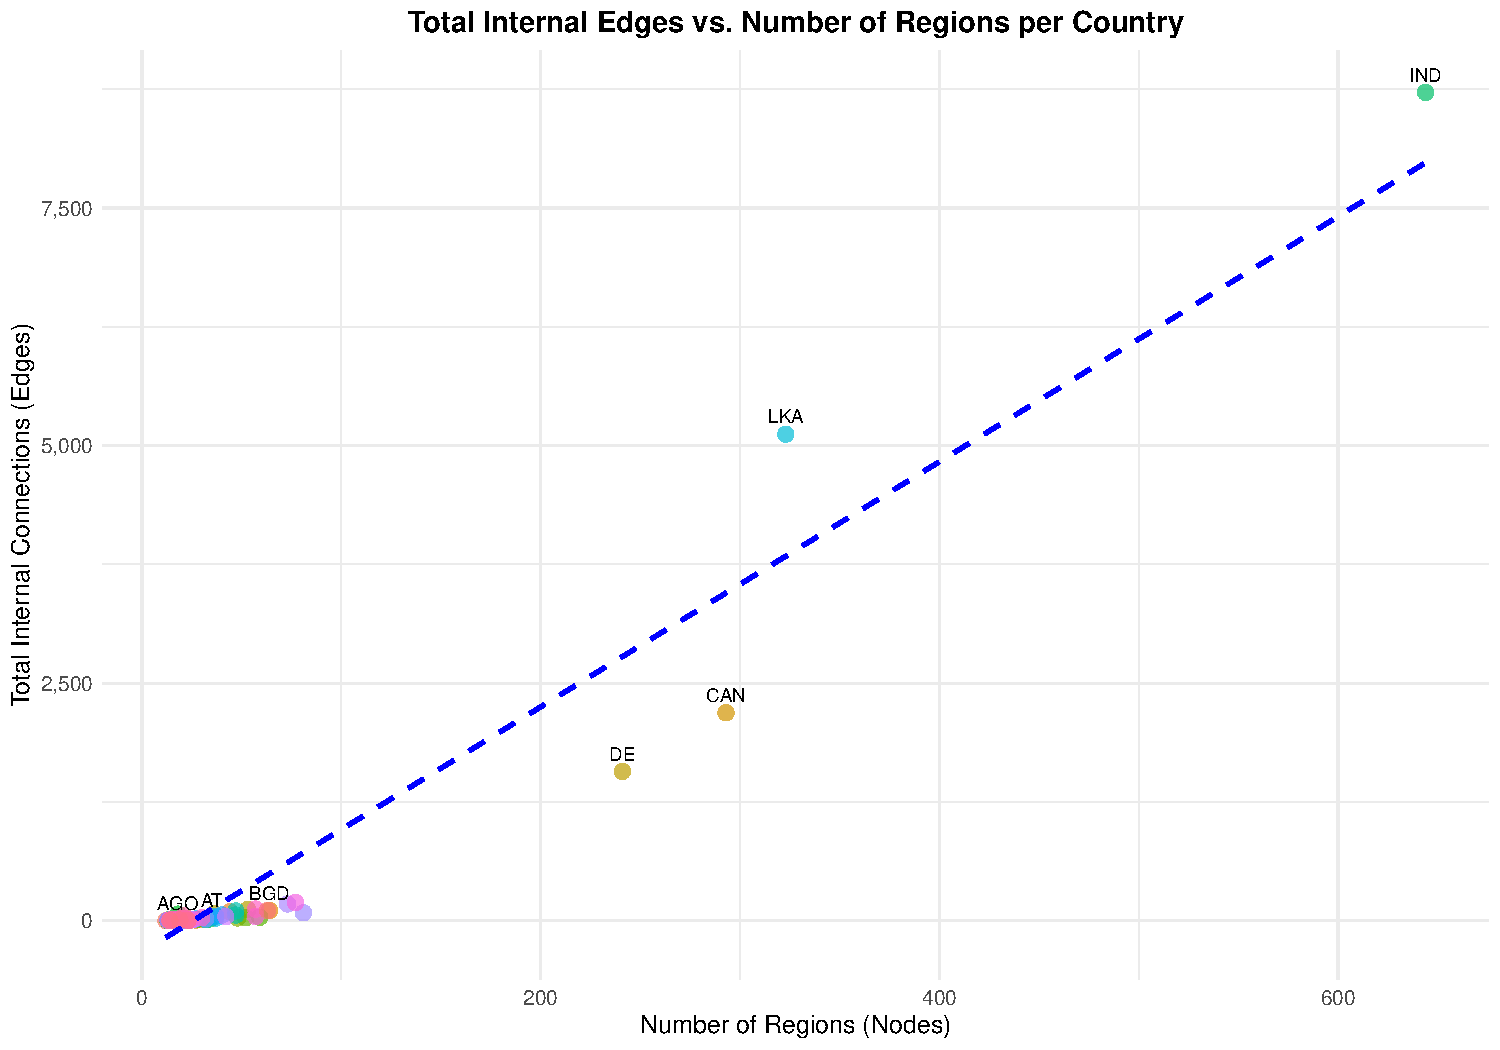
\includegraphics[width=0.75\textwidth]{images/edges_vs_nodes_plot.pdf}
  \caption{Number of nodes vs. number of edges across countries.}
  \label{fig:network-structure}
\end{figure}

\begin{figure}[h!]
    \centering
    \captionsetup[subfigure]{skip=2pt}
    \subfloat[India: Degree Distribution]{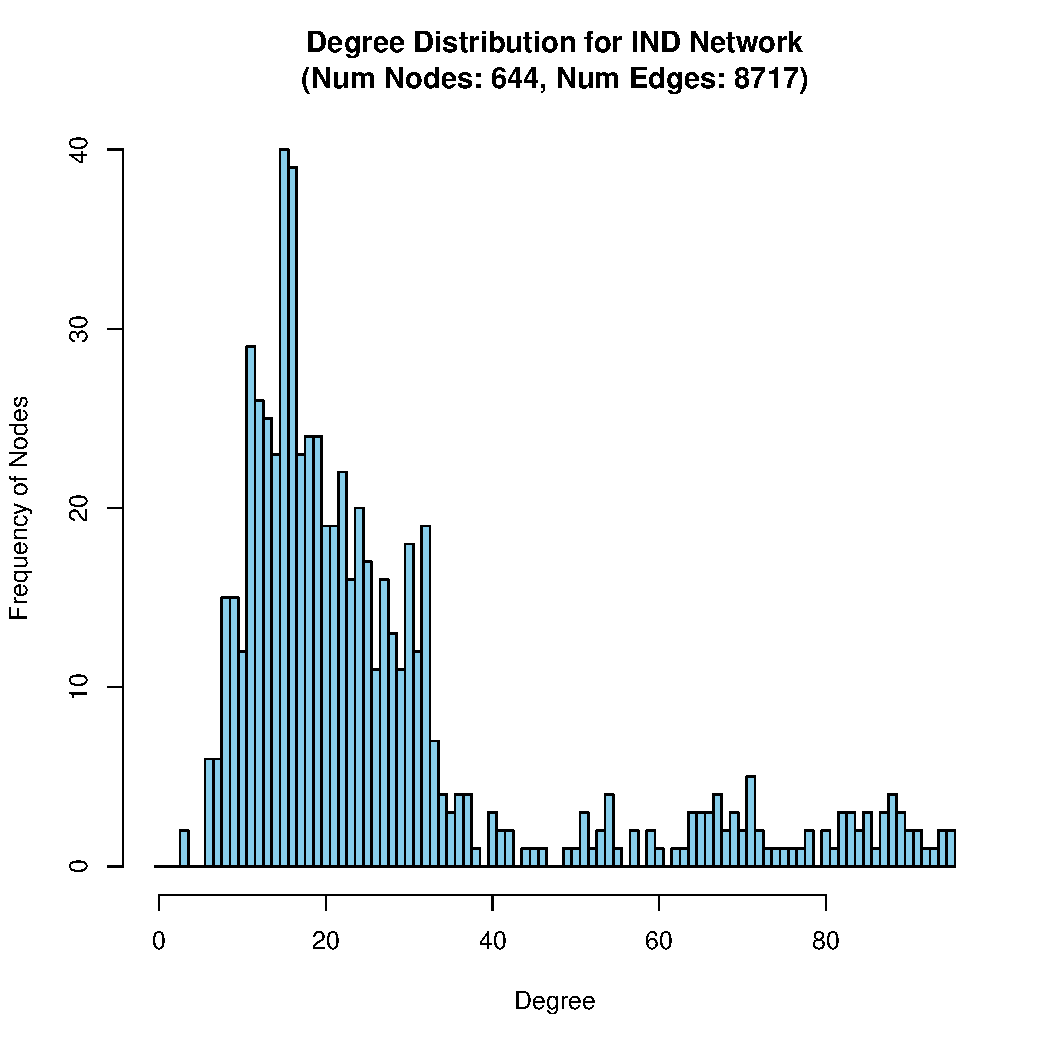
\includegraphics[width=0.48\textwidth, height=5cm]{images/IND_degree_distribution.pdf}}
    \hfill
    \subfloat[India: Network Topology]{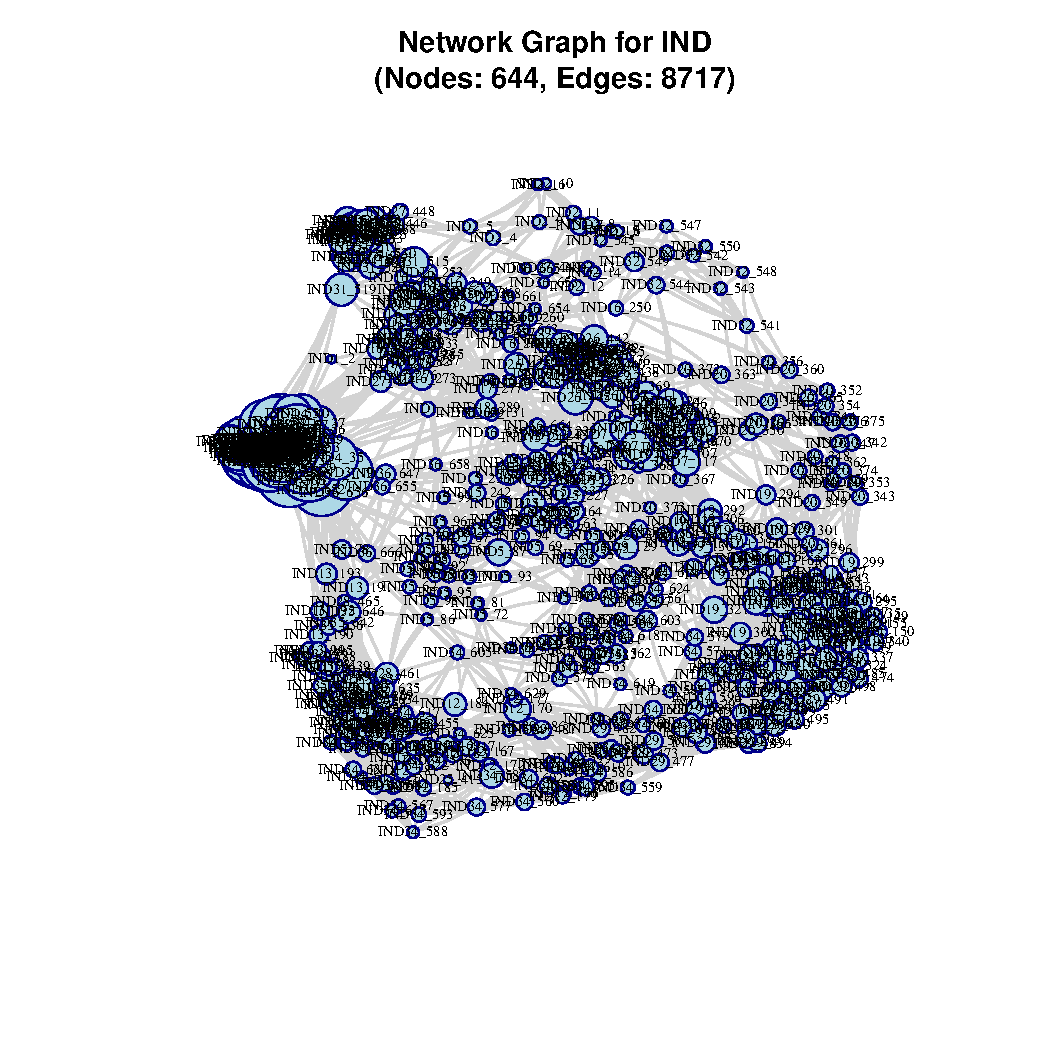
\includegraphics[width=0.48\textwidth, height=5cm]{images/IND_network_graph.pdf}}
    \vspace{0.1em}
    \subfloat[Serbia: Degree Distribution]{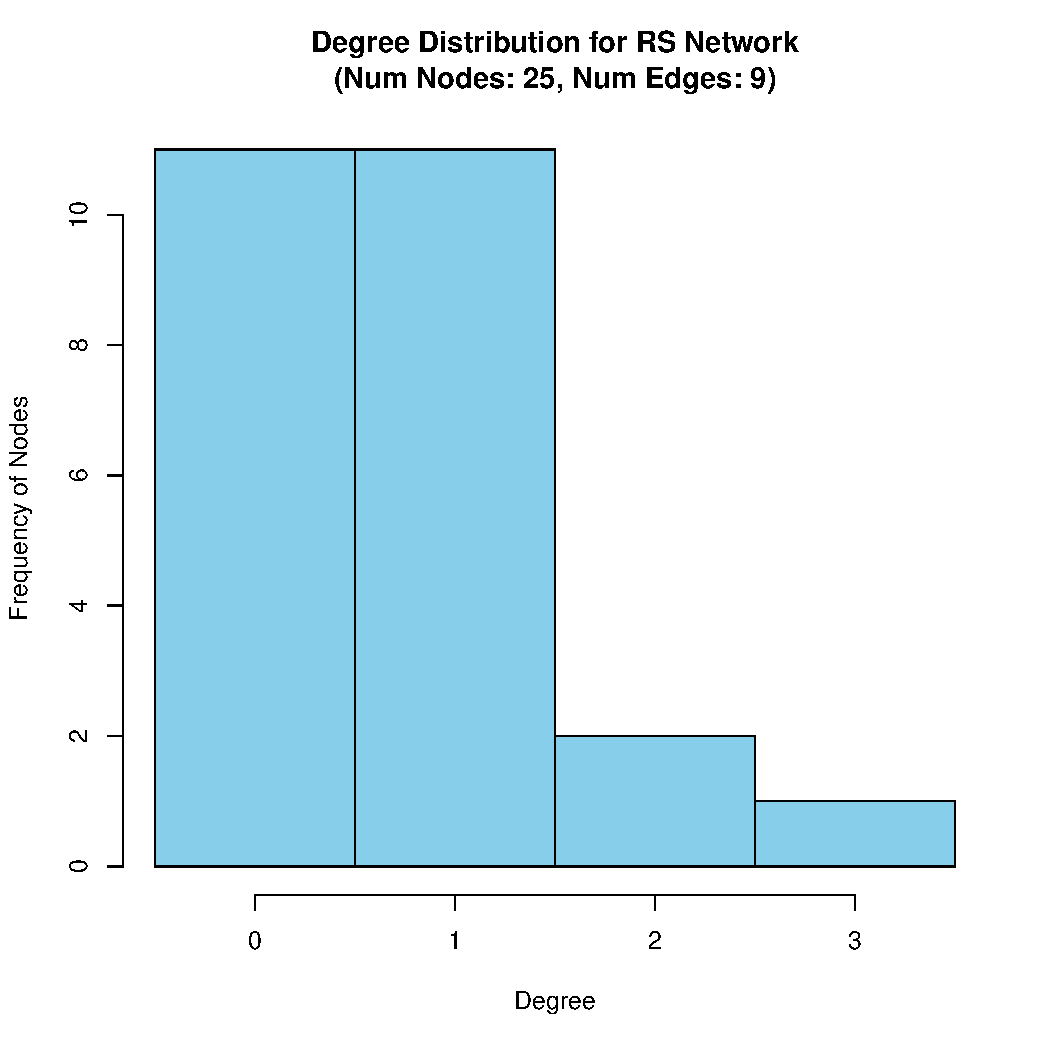
\includegraphics[width=0.44\textwidth, height=4.5cm]{images/RS_degree_distribution.pdf}}
    \hfill
    \subfloat[Serbia: Network Topology]{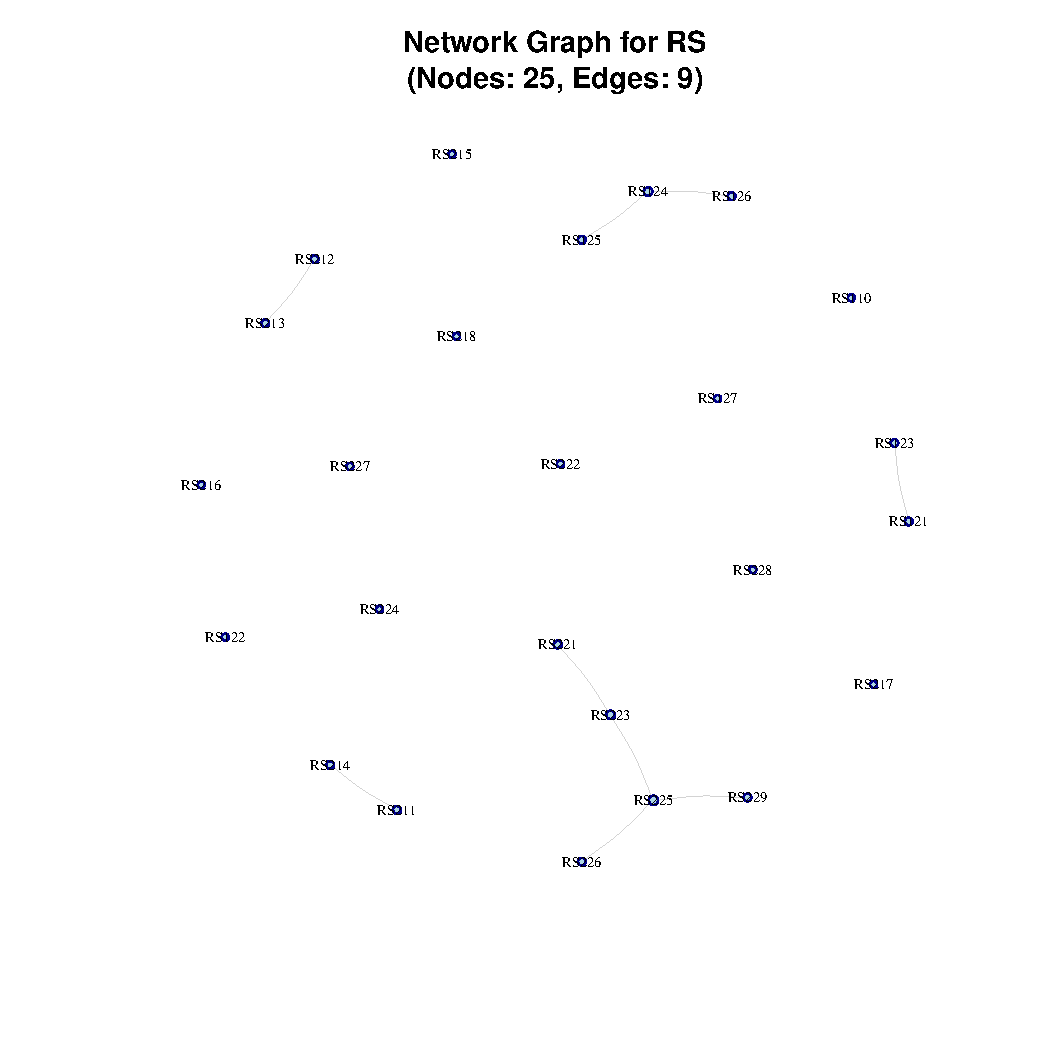
\includegraphics[width=0.44\textwidth, height=4.5cm]{images/RS_network_graph.pdf}}
    \caption{(a) India’s degree distribution, (b) India’s network, (c) Serbia’s degree distribution, (d) Serbia’s network.}
    \label{fig:combined_network_analysis}
\end{figure}